% !TeX program = platex
% Encoding: UTF-8
\PassOptionsToPackage{dvipdfmx}{color}
\documentclass[submit,techrep]{ipsj}
\usepackage[dvipdfmx]{graphicx}
\usepackage{url}
\usepackage{array}
\setcounter{year}{2026}
\providecommand{\newblock}{\hskip .11em plus .33em minus .07em}
\renewcommand{\doi}[1]{{\normalfont DOI: \urlstyle{same}\url{#1}}}
\begin{document}
\title{WebAssemblyクリプトジャッキングデータセットにおける\\難読化の影響分析と解析支援手法の検討}
\etitle{Obfuscation Effects and Analysis Support Approaches in WebAssembly Cryptojacking Datasets}
\affiliate{KIT}{金沢工業大学大学院\\Graduate School, Kanazawa Institute of Technology}
\author{貝沼英亮}{EISUKE KAINUMA}{KIT}[c6600873@st.kanazawa-it.ac.jp]
\author{向井宏明}{HIROAKI MUKAI}{KIT}[mukai.hiroaki@neptune.kanazawa-it.ac.jp]
\begin{abstract}
公開WebAssembly採掘データセットの変換機構・実行経路と，13件のハッシュ出力・速度・構造を照合した．xmr-wasmの平坦化版では命令数1.166倍，速度0.678倍となり，命令増加と速度低下の順序は命令置換版と一致しなかった．一部の変換箇所は測定入力で実行されない．解析支援の予備比較ではSWAMPED由来23バイナリを各6回測定し，評価入力の出力保持と単純変換の整理を確認したが，一貫した速度改善は得られなかった．局所正規化と読み取り専用解析の併用を候補として検討する．実世界の普及率や検知改善は示さない．
\end{abstract}
\begin{eabstract}
We relate obfuscation mechanisms and execution paths to outputs, throughput, and structure in 13 WebAssembly mining artifacts. Instruction growth does not rank throughput loss, and some transformed paths are skipped. A further six-repetition evaluation of 23 SWAMPED-derived artifacts preserves evaluated outputs and simplifies selected transformations, without consistent throughput improvement. We discuss local normalization and read-only analysis as limited support approaches. Deployment prevalence and detector improvements are not established.
\end{eabstract}
\maketitle

\section{はじめに}
WebAssembly（以下Wasm）はブラウザ等で実行できるバイナリ形式である\cite{webassembly}．Wasmは暗号資産のマイニング（採掘）にも用いられる．採掘機能を備えたプログラムと，利用者の同意なく計算資源を使うクリプトジャッキングは区別する必要がある．関連する公開データセットには，収集したWasmバイナリと，研究者が難読化などのコード変換を加えたバイナリが含まれる\cite{konoth2018,harnes2024,kim2025}．難読化とは，計算内容を保ちながらコードを書き換え，処理の内容を読み取りにくくすることである．既存研究では難読化手法や検出への影響を評価している．しかし，データセットに付されたラベルだけでは，コードのどこが変換され，測定時にどの処理が実行されるかは分からない．本稿では各Wasmバイナリの難読化の仕組みを調べ，出力の正しさを確認した上で，ハッシュ計算速度との関係を分析する．
\begin{description}
\item[RQ1] WebAssemblyの採掘用データセットで確認できる難読化手法とその仕組みは何か．通常の処理や研究用の計測コードとどう区別でき，データセットや実装によってどのような傾向があるか．
\item[RQ2] 難読化はハッシュ出力の正しさ，計算速度，コード構造・命令数・ファイルサイズにどのような影響を与えるか．その傾向は複数の採掘プログラムに共通するか．
\end{description}
コード変換の影響を調べるため，元のファイルと変換後のファイルを比較する．以下では，比較の基準となるファイルを「基準版」，変換後のファイルを「変換版」と呼ぶ．SWAMPEDの基準版は，今回の難読化を適用する前のバイナリである．
同じファイルと入力条件に基づき，RQ1の変換箇所とRQ2の出力，速度，コード構造を照合し，次の知見を得た．
\begin{enumerate}
\item xmr-wasmで命令増加と速度低下の順序が一致しない例と，測定入力では実行されない変換箇所を示した．
\item SWAMPEDを同条件で比較し，命令増加と出力保持を確認したが，速度差は測定変動と重なった．
\item 設定と命令列を照合し，通常・計測コードとの違い，ラベルや最適化条件の不一致を区別した．
\item 局所正規化と式・状態モデルを予備比較し，23バイナリの6反復で構造の整理と速度改善の違いを示し，解析支援を検討した．
\end{enumerate}
新しい難読化アルゴリズムや検出回避能力は評価しない．データセットの収録数から，実際の攻撃で各手法が使われる割合は推定しない．また，データセット名が異なるだけでは独立した実装とはみなさない．


\section{関連研究と本研究の貢献}
Cryptic Bytesは，ソースコード，LLVM中間表現（IR），Wasmの各段階で変換と検出を扱い，100秒間のハッシュ計算速度も評価している\cite{harnes2024}．WebAssembly diversification for malware evasionも，通常版6件・変換版120件について約1000秒間の測定とマイニングプールでの検証を行っている\cite{cabrera2023}．MineSweeperの表10は，Wasmとasm.jsの違いやCPU利用率による速度差を扱う\cite{konoth2018}．したがって，採掘用Wasmの難読化後の速度測定は本研究が初めてではない．既存研究によるプールでの検証を踏まえ，本稿では公開された入力データを用い，ネットワークを無効にしたローカル環境で追加測定を行う．

Proof-of-Theftの確認した本文・補足には，出力照合と反復ハッシュ速度を組み合わせた報告はなかった\cite{sermchaiwong2026}．ただし配布物にhashrate.jsがあり，過去の測定未実施とは断定できない．本稿は配布2実装の機構・出力・速度を対応付ける．SWAMPED第IV.D節はホスト側関数を空の関数で置き換えて時間を測る\cite{kim2025}．本稿は必要なホスト処理を用意し，全体ハッシュの期待値一致を伴う比較を行う．

MinerRay第6.4節・表5は検出グラフの構築・走査時間で，採掘速度ではない\cite{romano2020minerray}．WASMixerのarXiv第1版はブラウザ依存を理由に採掘用D3を時間評価から除外する\cite{cao2023}が，刊行版\cite{cao2024published}との照合は未完了である．今回のSWAMPED入力は両データセットにも同じSHAで収録されるが，今回の変換はSWAMPEDのコードによる．通常・計測コードの比較にはWasmBench\cite{hilbig2021}とSEISMIC\cite{wang2018seismic}を用いる．判断は確認した一次資料に限る．

本研究は未報告の測定値だけを新規性とせず，変換機構・入力条件と測定値を対応付け，解析支援の適用範囲を評価する．全実行経路や速度差の原因を確定したものではない．

\section{対象と分析方法}
\subsection{対象ファイルと比較の方法}
採掘に関する先行研究の公開データセットのうち，Wasmバイナリを入手できたものを対象とする．Cryptic Bytesでは，CryptoNight系列の10プログラムについて，未最適化・最適化済みの2条件で配布された20,460件を基準版と対応付けた．対象には，比較の基準となるバイナリ，LLVMとTigressの各8設定，wasm-mutateによる変換，基準版を自身と比較する20件が含まれる．対象には互いに関連する派生実装が含まれるため，独立した10系統のマルウェアとしては扱わない．Proof-of-Theftでは，34ディレクトリを9設定に整理した．元のバイナリ，中間生成物，Wasabiで計測用コードを追加したバイナリが混在するため，origという名前だけでは，変換前のファイルと判断できない．

収集ファイルのうち，MineSweeperのminer samples 34種類中33種類，SWAMPEDのCryptojackers 43種類中42種類を静的解析できた．WasmMalの悪性・良性の区分は公開元の分類に従うものであり，悪性とされた全ファイルで採掘機能を確認したわけではない．比較用の良性グループとWasmBenchを含め，各コード特徴の出現割合を表\ref{tab:features}に示す．各グループ内ではSHA-256値が同じバイナリを重複としてまとめるが，グループ間の重複は残している．SWAMPEDのWasmバイナリ42種類中35種類は，他の取得記録にも収録されていた．この結果から，攻撃全体で難読化が使われる割合は推定しない．

\begin{table*}[t]
\caption{各コード特徴を含むファイルの割合（分母は解析できたファイル数，単位\%）}
\label{tab:features}
\centering\small
\begin{tabular}{lrrrrr}
\hline
データセット & \shortstack{解析済みの種類数／\\取得した種類数} & \shortstack{ループ内の\\分岐表} & 間接呼び出し & nop命令 & \shortstack{難読化手法の\\確認割合} \\
\hline
MineSweeper／miner samples & 33／34 & 33.33 & 100.00 & 54.55 & 推定せず \\
SWAMPED／Cryptojackers & 42／43 & 42.86 & 100.00 & 57.14 & 推定せず \\
WasmMal／malware（参考） & 7,510／7,512 & 46.07 & 98.88 & 59.57 & 推定せず \\
WasmMal／benign（比較） & 7,510／7,512 & 52.77 & 81.85 & 20.27 & 推定せず \\
WasmBench／filtered（比較） & 8,449／8,460 & 56.66 & 82.73 & 25.79 & 推定せず \\
\hline
\end{tabular}
\end{table*}

\subsection{難読化の仕組みとコード構造の解析}
SHA-256，取得元のリビジョン，生成設定，基準版との対応を保存し，WebAssembly Binary Toolkit（WABT）1.0.42で検証・逆アセンブルする．Wasmテキスト形式（WAT）の命令列から，関数数，命令数，ループ内の分岐表（\texttt{br\_table}），直接・間接呼出し，ロード・ストア，各セクションの大きさを調べる．検証失敗は解析不能とし，特徴なしとは扱わない．ラベル，特徴，確認した機構を区別し，状態値の生成・更新と処理の戻り先，仮想命令の読出し，同値な算術式を追跡する．全関数の動作同一性や自動分類の精度は評価しない．

基準版は比較の基準であり，難読化がないことを保証しない．差分$\Delta X=X-X_0$と比$r_X=X/X_0$を求め，基準値0では差分だけを残す．Cryptic Bytesはプログラム・最適化条件・変換設定ごとに中央値を求め，10本の分布を示す．同じ最適化条件の基準版と比べ，多数の派生版を独立した事例として統計検定に用いない．wasm-mutateの混在変換は単一手法の効果と解釈しない．静的命令数はコード上の個数であり，実行回数やメモリ使用量ではない．

\subsection{出力と実行速度の測定}
ローカルでの反復測定は，Proof-of-Theftのwebminerpoolhashcn・xmr-wasm各5件，SWAMPED入力1件と今回の変換版2件の計13件を対象とする．SHA-256でRQ1と対応付け，Wasabi計測版を除く．Windows上のネットワーク無効Linuxコンテナ，Intel Core i9-11900K，Node.js v18.20.4，V8 10.2.154.26-node.37，ワーカー1を使う．配布JavaScriptまたはインポート情報に基づくホスト処理から同期呼出しし，初期化は測定外とする．呼出しループを含む速度であり，Wasm命令だけの速度ではない．

出力の検証には，入力と期待出力の組であるテストベクトルを用いる．期待出力には，XMRig v6.18.0の\texttt{CryptoNight\_test.h}で公開されているv0の入力5件に対応する値を用いる\cite{xmrigvectors}．xmr-wasmでは入力の先頭バイトからvariant（アルゴリズムの種類）を選ぶため，v0に対応する3件を使う．target（ハッシュ値を判定するしきい値）を最大値に設定し，nonce（採掘で変化させる値）が変わらないことと，1回のハッシュ計算の出力が一致することを確認する．webminerpoolhashcnのcn-picoの測定では，過去にマイニングプールで受理された13件のジョブ，nonce，出力を照合する．新たにプールへ結果を送信するものではない．限られた入力で出力が一致したことと，すべての入力で変換前後の動作が同じであることは区別する．解析支援の追加実験では，同じSWAMPED入力から得た23バイナリを，3秒以上のウォームアップ後，各30秒以上・6反復で測定した．対象と照合条件は第6.1節に示す．

計算速度は，完了したハッシュ計算数を経過時間で割ったハッシュレートで表す．単位は毎秒のハッシュ計算数を表すH/sとする．測定前にはプログラムを一定時間動かすウォームアップを行う．webminerpoolhashcnでは1秒間のウォームアップ後，各5秒間の予備測定を3回繰り返す．xmr-wasmとSWAMPEDの基準版・変換版では，3秒間のウォームアップ後，各30秒以上の測定を3回繰り返す．測定回ごとにファイルの実行順をずらし，最終出力を確認する．結果には中央値，最小値から最大値までの範囲，同じ測定回の基準版に対する比を示す．各ファイルは順番に測定するため，同じ測定回でも測定時刻は異なる．また，最小値から最大値までの範囲は信頼区間を表さない．

\section{RQ1：確認した難読化の仕組みとデータセットの傾向}
\subsection{難読化と通常の処理・計測用コードの違い}
研究用に公開されたバイナリには，制御フロー平坦化，偽の制御フローの追加，分割，算術式や定数の変換，関数呼び出しの変更，コードの仮想化などが含まれる．制御フロー平坦化（以下，平坦化）は，状態値で次に実行する処理を選ぶように，処理の流れを変える手法である．コードの仮想化（以下，仮想化）は，独自に定義した命令列を解釈して実行する形に変換する手法である．Cryptic Bytesの各設定には10本$\times$2条件のファイルがある．一方，Proof-of-Theftでは設定ごとの収録内容が均等ではない．データセットのラベルから分かる手法と，命令列で仕組みを確認できた手法は分けて整理する．

Cryptic Bytesのcn-0では，エクスポートされた関数名\texttt{hash\_cn}を使って，基準版と変換版の関数を対応付けた．Tigressのflatten設定で変換した版は，状態の初期値5を保存し，12要素の分岐表で処理を選んだ後，状態を更新して共通のループへ戻る．virtualize設定で変換した版は，仮想命令の読み出し位置を指すポインタから1バイトを読み，その値から16を引いて233要素の分岐表へ渡す．読み出し位置を1または4進める処理があり，状態値で処理を選ぶ平坦化とは区別できる．全仮想命令の意味は復元していない．

LLVM subobf版では$x\ll3$が次の式へ変わる．
\[
(x\mathbin{\&}\mathord{\sim}8)(\mathord{\sim}x\mathbin{\&}8)
+(x\mathbin{|}8)(x\mathbin{\&}8).
\]
$u=x\mathbin{\&}\mathord{\sim}8$，$v=x\mathbin{\&}8\in\{0,8\}$とすると，式は$u(8-v)+(u+8)v=8x$となる．32ビットの範囲を超えた桁を捨てて計算すると，元のシフトと一致する．antialiasanalysis設定の版では，メモリから読み出した番号を間接呼び出しに使う箇所があった．この設定が対象とするエイリアス解析とは，異なる参照が同じメモリ領域を指すかを調べる解析である．ただし，基準版の対応箇所との差はまだ確定していないため，この処理が難読化によって追加されたとは断定しない．

\label{sec:rq1-controls}
難読化していない処理にも，同じような特徴が見られる．CreaturePackの分岐表は数値に応じて処理を選ぶもので，状態の更新やループを伴わない．これは，WASMixerのbase64-cliに見られる，状態を更新して共通の選択ループへ戻る構造とは異なる．xmr-wasmの基準版にある70箇所の分岐表は，同梱されたCryptoNightRで演算を選ぶ処理に対応する．cryptonight-hashの基準版にある間接呼び出しも，内部状態に応じてBlake，Groestl，JH，Skeinを選ぶ通常の最終処理である．このため，分岐表や間接呼び出しがあるだけでは難読化と判定できない．

WasmMalでは，悪性と分類された121件，良性と分類された3件に，SEISMICの計測用関数と一致する関数があった．A-StarとCreaturePackでは，カウンタを更新する命令を取り除くと，元の147・756関数すべての命令列とそれぞれ一致した．これらは，命令数が計測処理によって増える例として比較に用い，採掘ファイルで難読化を確認した件数には含めない．表\ref{tab:features}の割合も，各コード特徴の有無を示すものであり，難読化手法を確認できた割合ではない．

\subsection{実測した13件のファイルの難読化と実行経路}
\label{sec:proof-mechanisms}
webminerpoolhashcnでは，基準版と4種類の変換版のディレクトリにあるすべてのMakefileで，\texttt{-enable-bcfobf}が指定されていた．当時のファイル生成手順を確定できないため，ディレクトリ名だけを根拠に手法を特定しない．xmr-wasmでは，名前に対応するコンパイルオプションがあり，同梱されたC/C++ソースとヘッダ計46件のファイルのSHA-256値も一致した．ただし，当時使われたコンパイラや生成されたオブジェクトファイルまで同じとは確認できていない．分割設定は，途中に分岐を含まない命令列であるLLVMの基本ブロックを，より小さく分ける基本ブロック分割を指す\cite{emccobfdocs}が，変換前後の中間表現は入手できていない．Wasm内の命令の配置やblock命令による構造の変化だけでは，実際にその変換が適用されたかを確定できない．偽の制御フローの追加についても，仕組みは未確認とする．

xmr-wasmの平坦化版では，外部から呼び出せるhash関数，XORの補助関数112・118，初期化を行う関数83，鍵を取り込む関数82，解放処理を行う関数86で，状態に応じた処理の選択，状態の更新，共通ループへの復帰を確認した．hash関数には分岐表がなく，分岐表を使わない平坦化を確認できる．関数111から補助関数118への2箇所の呼び出しはメインループ内にあるが，初期化などはループの外にある．実行時の呼び出し回数や，各処理が実行時間に占める割合は測定していない．

関数113への呼び出しはvariant 4以上に限られ，今回のv0入力では実行されない．平坦化版の関数111では，この未実行のブロック内で命令列が9,428行増えていた．一方，それ以外の3,609行は，ローカル変数とラベルの名前を対応付けると一致した．そのため，増えた行数をv0の実行時に追加された命令数とはみなせない．ただし，呼び出し先やローカル変数の宣言の変化，JIT（Just-In-Time）コンパイル，コード配置の影響は残る．JITコンパイルは，実行時にコードを機械語へ変換する処理である．

命令置換版では，外部から呼び出せるhash関数に，$(x-C)-6+C=x-6$と$n-(0-1)=n+1$になる式を確認した．ただし，今回の入力でtargetを最大値に設定した条件では，どちらの処理も実行されない．一方，呼び出し先の関数111の二重ループでは，先に示した式の8を16に替えた，$x\ll4$と同じ計算結果になる変換を確認した．外部呼び出しを仲介するラッパー関数と内部の計算処理で命令置換を確認したが，すべての実行経路を確認したわけではない．

SWAMPEDのWasmバイナリから今回作成した変換版では，nop挿入を30関数の3,089箇所，整数定数の分割を29関数の542箇所で行ったことを記録した．nopは何も処理しない命令である．挿入したnopを取り除き，分割した式を元に戻すと，モジュール全体のWATが基準版と一致した．計測用コードは追加していない．データセットの公開元が作成した変換版と，今回作成した変換版は区別する．

\subsection{RQ1への回答}
複数の設定を調べ，処理の流れ，算術式，関数呼び出しを変える手法を確認した．ただし，確認した仕組みと適用範囲はバイナリによって異なる．速度を測定したファイルでは，平坦化や命令置換の箇所，今回のnop挿入と整数定数の分割を命令列で確認し，通常の暗号処理や計測用コードと区別した．名称と設定が一致しない場合や仕組みを確認できていない場合は，ファイルに変化があっても，特定の難読化手法の効果とはみなさない．収集したバイナリ全体に占める各難読化手法の割合は未確定である．

\section{RQ2：コード構造，出力の正しさ，計算速度}
\subsection{Cryptic Bytesの静的解析による比較}
\begin{figure*}[t]
\centering
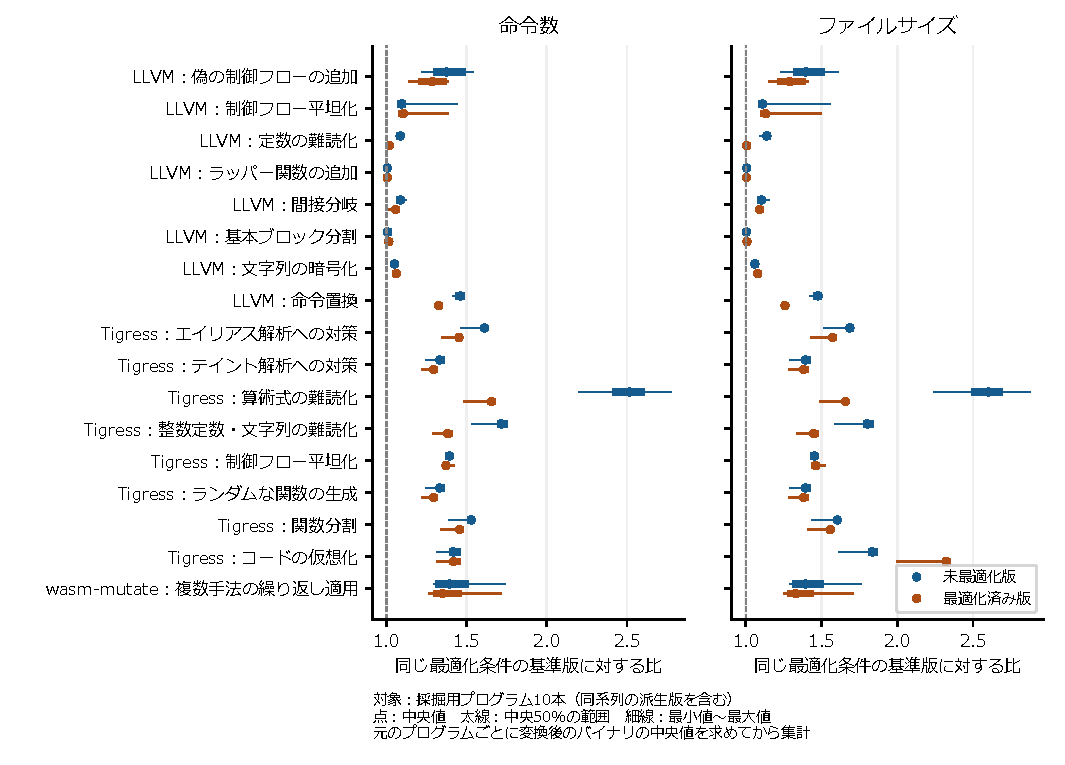
\includegraphics[width=0.82\textwidth]{../results/mining-methods/figures/method-size-instructions.pdf}
\caption{Cryptic Bytesの命令数とファイルサイズの比．元のプログラム10本について，同じ最適化条件の基準版に対する比の分布を示す．手法名はデータセットの公開元の設定に基づく．}
\label{fig:methods}
\end{figure*}
全20,460件を解析した結果，図\ref{fig:methods}のように，手法と最適化条件によって命令数やサイズの増加量が異なった．未最適化版の命令数の比の中央値は，Tigressの算術式の難読化設定encodearithmeticで2.515，LLVMの命令置換設定subobfで1.461だった．平坦化ではLLVMが1.098，Tigressが1.394となった．最適化済み版のencodearithmeticとsubobfでは，それぞれ1.655・1.327だった．同じ手法名でも変換する段階や範囲が異なるため，これらの値だけでは手法の優劣を示せない．

仮想化設定virtualizeによる命令数の比は，未最適化版1.417，最適化済み版1.418と近かったが，ファイルサイズの比は1.834・2.322と異なった．cn-0の変換前後のファイルを比べると，未最適化版ではcode・dataセクションがそれぞれ165,827・97,625バイト増え，最適化済み版ではそれぞれ86,969・97,598バイト増えていた．codeセクションには命令，dataセクションにはデータを格納する．この変化は仮想命令列を持つ仕組みと矛盾しないが，dataセクションの全内容を仮想命令として復元したわけではない．サイズの比には，基準版の大きさも影響する．

Tigressの平坦化では，いずれの最適化条件でもループ内の分岐表が中央値で70増え，未最適化版のストア命令は6,733増えた．antialiasanalysis設定では，直接呼び出しが218減り，間接呼び出しが358増えた．減少数と増加数は一致せず，一対一で置き換わったわけではない．比較対象の基準版と変換版にはいずれもnameセクションがなく，名前情報を削除する変換の効果は評価できない．以上は静的解析で確認した構造の変化である．次節では，実行速度の測定結果と照合する．

\subsection{Proof-of-Theftの出力と速度}
\label{sec:runtime}
webminerpoolhashcnの5件では，公開されたv0のテスト入力5件について，計算した出力がすべて期待値と一致した．cn-picoについても，保存していた受理済み出力13件とすべて一致した．各5秒間の測定を3回繰り返した速度の中央値は，基準版204.04，平坦化版213.29，分割版222.99，命令置換版225.20，偽の制御フロー版212.24 H/sだった．ここでの変換版の名称は，データセットのラベルに従う．名前と設定が一致せず，測定時間も短いため，これらの差を4手法による高速化や追加の負荷とは解釈しない．

\label{sec:xmr-runtime}
xmr-wasmの5件でも，公開されたv0のテスト入力3件の出力が期待値と一致した．各30秒以上の測定を3回繰り返した結果を表\ref{tab:xmr-runtime}に示す．計15回の測定すべてで，最終出力の一致とnonceが変わらないことを確認した．
\begin{table}[t]
\centering\small
\caption{xmr-wasmの計算速度と命令数の比（各30秒以上，3回測定）．比は基準版に対する値．偽の制御フロー版は最適化条件が異なる．}
\label{tab:xmr-runtime}
\setlength{\tabcolsep}{2.8pt}
\begin{tabular}{lrrr}
\hline
変換設定名 & \shortstack{計算速度の\\中央値（H/s）} & \shortstack{最小値～最大値\\（H/s）} & \shortstack{命令数\\の比} \\
\hline
基準版 & 9.11 & 8.50--9.34 & 1.000 \\
平坦化 & 6.18 & 5.86--6.22 & 1.166 \\
\shortstack[l]{基本ブロック\\分割（設定名）} & 8.59 & 8.46--9.01 & 1.033 \\
命令置換（設定名） & 6.72 & 6.61--6.82 & 1.655 \\
\shortstack[l]{偽の制御フロー\\（$-O2$）} & 23.08 & 22.69--24.05 & 0.413 \\
\hline
\end{tabular}
\end{table}
平坦化版では，基準版に対して命令数が1.166倍，サイズが1.170倍となり，速度の中央値の比は0.678だった．命令置換と表記された版では，命令数が1.655倍，サイズが1.641倍，速度の比が0.738となった．このように，命令数の増加量と速度低下の大きさは必ずしも対応しない．同じ測定回の基準版に対する速度の比は，平坦化版0.661--0.689，命令置換版0.708--0.790で，両版とも3回の測定すべてで1未満だった．ただし，当時のビルド条件や変換の適用範囲を完全にそろえた比較ではないため，難読化の仕組みだけでは速度低下をすべて説明できない．

基本ブロック分割と表記された版では速度の比が0.943だったが，同じ測定回の基準版に対する比は0.906--1.011となり，基準版より速い回と遅い回があった．偽の制御フローと表記された版では，速度の比が2.534，命令数の比が0.413だった．ただし，この版だけに\texttt{-O2}が明示されているため，難読化によって高速化したとは結論しない．また，webminerpoolhashcnとは実装，アルゴリズム，呼び出し条件が異なるため，速度の絶対値は比較しない．

実行できなかったファイルは，出力不一致や速度0 H/sとは区別する．選定したProof-of-Theftの19件のうち，上記10件は出力を照合できた．一方，Tigressで手法を併用した版と仮想化版は，間接呼び出しで実行時エラーになり，原因はまだ確定していない．cryptonight-hashの7件では，入力ごとに外部から呼び出す関数を確認できなかった．内部関数のABI（引数などを受け渡すための規約）の一部と，一部の平坦化を静的解析で確認した段階であり，出力と速度の実測には含めていない．

\subsection{SWAMPEDの難読化前後の比較}
\label{sec:swamped-hash}
\label{sec:swamped-controlled}
取得した42件について，エクスポートされた関数やホスト側の処理への依存を調べた．そのうち，SHA-256値が\texttt{046dc081}で始まるファイルの\texttt{\_cryptonight\_create}と\texttt{\_cryptonight\_hash\_variant\_0}を呼び出した．元のJavaScriptがないため，命令列から旧Emscriptenのメモリ・テーブル・時刻・UTC変換・プロセスIDを実装した．初期メモリは16 MiBで，未対応呼出しはエラーとし，空の関数で代用しない．元のホストの完全再現ではない．公開されたv0のテスト入力5件では，出力がすべて期待値と一致した．このファイルはMinerRay，WasmBench，WASMixer，WasmMalにも同じSHA-256値で収録されており，独立した5件ではない．

公開された変換コードのコミット\texttt{04e2bcc}を用い，変換処理の本体を変えずにWATを扱えるようアダプタを用意して，nop挿入版と整数定数の分割版を作成した．挿入位置の選択にはベータ分布beta(1,1)を用い，各関数の候補箇所のうち0.1の割合を選び，最低1箇所は選択するという元の規則に従った．乱数生成器も固定した．浮動小数点定数の丸め誤差を避けるため，variant\_2関数は定数分割の対象から除外した．整数定数$c$を，$a+b=c$となる加算の式に置き換える．例えば，\texttt{i64.const 0}は$-1+1$を計算する命令列となる．

基準版と変換版は，同じWABTを使い，Wasmテキスト形式からバイナリを生成した．基準版と元の公開バイナリのSHA-256値は一致した．3件のファイルすべてについて公開された入力5件の出力とインポート・エクスポートの一覧を確認し，ホスト環境，メモリ，入力，初期時刻を同じにして繰り返し測定した．計9回の測定すべてで最終出力が一致し，測定後に確認した5件の出力も一致した．追加評価では外部通信やプールへの送信を行わず，報酬も発生させない．
\begin{table}[t]
\centering\small
\caption{SWAMPEDの基準版と変換版の比較（同じ条件で各30秒以上，3回測定）}
\label{tab:swamped-controlled}
\setlength{\tabcolsep}{3.5pt}
\begin{tabular}{lrrr}
\hline
変換内容 & \shortstack{計算速度の\\中央値（H/s）} & \shortstack{最小値～最大値\\（H/s）} & \shortstack{命令数\\の比} \\
\hline
基準版 & 32.39 & 27.09--32.73 & 1.000 \\
nop挿入 & 31.08 & 29.56--32.72 & 1.097 \\
整数定数の分割 & 31.53 & 28.94--32.08 & 1.034 \\
\hline
\end{tabular}
\end{table}
\begin{figure*}[t]
\centering
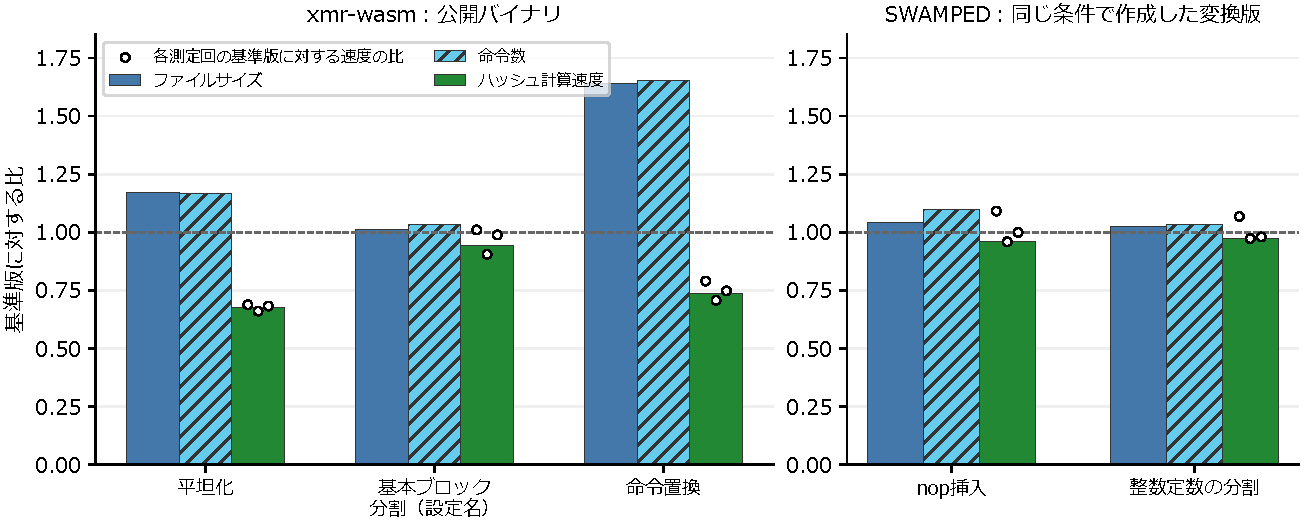
\includegraphics[width=\textwidth]{../results/runtime-mining/cross-dataset/hash-structure-comparison.pdf}
\caption{基準版に対するファイルサイズ・命令数・計算速度の比．左はxmr-wasmの公開バイナリ，右はSWAMPEDのWasmバイナリから作成した変換版．計算速度の棒は中央値の比，白丸は各測定回の基準版に対する比で，3回の結果を示す．ファイルは順番に測定しており，白丸は信頼区間ではない．最適化条件が異なる偽の制御フロー版は表だけに示す．}
\label{fig:swamped-controlled}
\end{figure*}
nop挿入版では，ファイルサイズの比，命令数の比，速度の中央値の比が，それぞれ1.042・1.097・0.960となった．整数定数の分割版では1.024・1.034・0.973だった．測定値の範囲は基準版と重なり，同じ測定回の基準版に対する速度の比もnop挿入版0.960--1.091，整数定数の分割版0.973--1.068となった．どちらも基準版より速い回と遅い回がある．基準版自体も，1回目の27.09 H/sから3回目の32.73 H/sへ20.8\%上昇した．実行順を変えても，時間経過に伴う変動は取り除けない．そのため，速度の中央値のわずかな低下を，難読化による負荷の増加と断定することはできない．Wasmエンジンが追加命令を除去した可能性はあるが，生成された機械語を確認していないため断定しない．

\subsection{RQ2への回答}
評価入力では変換版も期待出力と一致した．xmr-wasmでは命令増加と速度低下の順序が一致せず，SWAMPEDでは速度差が測定変動と重なった．実装に共通する傾向や手法単独の効果は未確定で，条件の異なる実装間の速度順位は付けない．

\section{考察と限界}
\subsection{変換機構に基づく解析支援手法の検討}
RQ1の機構とRQ2の結果を根拠に，局所正規化と読み取り専用解析を予備比較した．関数内のnop除去と連続整数定数のadd/sub/mul/and/or/xorの畳み込みを実装し，個別・併用をBinaryen 133の局所pass（vacuum，precompute）・O2と比較した．32・64ビットの剰余を用い，副作用・分岐を挟む式は変更せず，基準版・SHA・変換位置ログを判定に使わない．

SWAMPED開発2版と別乱数2設定・割合0.05／0.25の8版は，併用後に基準とバイト一致した．定数分割は既存最適化でも一致し，専用規則固有の効果ではない．最適化したnop版の残差は他命令だった．別12標本では通常・計測のA-Star・CreaturePack 4件は変更されず，通常base64-cli・seqtkの定数式も簡約されたため，規則適用を悪性判定に使えない．平坦化・複雑な置換の差は残った．専用72条件は署名・リソース宣言を保持したが，型保持だけで意味保存は保証しない．

追加評価では開発3入力・別乱数等9入力に6処理を適用した72条件を23SHAにまとめ，各6回，計138回測定した．同一SHAは測定を共有し独立標本数を増やさない．ホスト・入力・初期時刻・1ワーカーを固定し順序を回転した．全対象で公表5入力，追加12入力，測定前後・最終出力を照合した．基準の1／8／32バイト入力は再利用履歴により出力が異なり，原因は未特定である．追加分は除外せず，新規コンテキスト同士と同履歴・同順序の基準と比較した．独立期待値による正しさの確認は公表5入力に限る．

\begin{table}[t]
\centering\small
\caption{解析支援の追加実験における開発条件の速度中央値（H/s，各30秒以上，6反復）．同一SHAの条件は測定を共有する．}
\label{tab:normalization-runtime}
\setlength{\tabcolsep}{3pt}
\begin{tabular}{lrrr}
\hline
処理 & 基準版 & nop挿入版 & 定数分割版 \\
\hline
未処理 & 31.49 & 30.65 & 31.67 \\
両規則 & 31.49 & 31.49 & 31.49 \\
Binaryen局所 & 31.74 & 31.41 & 31.74 \\
Binaryen O2 & 31.36 & 31.10 & 31.36 \\
\hline
\end{tabular}
\end{table}
両規則後／未処理の中央値比はnop版1.0276，定数分割版0.9943，別乱数8版0.9827--1.0120で，基準自身も26.55--32.08 H/sに変動した（表\ref{tab:normalization-runtime}）．別乱数nop版は命令数が24.29\%増えても速度比0.9997・1.0037だった．構造の整理から一貫した高速化は導けず，同処理基準との比較でも専用規則の速度優位性は確認できない．6入力・各6反復の起動・入出力・検証込みの前処理時間も，専用120.1--781.1 ms，局所最適化36.6--171.7 msで専用が長かった．

複雑な置換にはMBA-Blast等\cite{liumba2021}を踏まえ，独立変数1個のビットをBoolean変数とする多項式でシフトとの対応を比較した．12～80ノードに限定し，分岐・メモリ・呼出しで依存伝播を切る．xmrで43出力，Cryptic Bytesの10プログラム・3設定・2ビルドの60件中，未最適化LLVM版10件で140出力を得た．重複を含む計183式・19,398有限入力は独立整数評価器と一致した．多入力のTigress候補5,018件は対象外で，最適化後の識別0件も完全除去を意味しない．

平坦化は既知の8・16バイトXORの4状態モデルを使う限定対照とした．通常・平坦化4関数の698ケース・1,396呼出しで，出力と一時スタック32バイトを除くメモリが一致した．自動復元や全モジュールの証明ではない．

専用72条件の10条件でnopの有無が消え，36条件で命令総数が変わった．原特徴が失われ得るため，原本・正規化結果・適用記録の併用が考えられる．固定MINOS公開重みを静的推論し，独立NumPy計算8入力と照合した．画素尺度0～255と0～1では144条件中21条件で予測が変わり，専用72条件の正規化前後のクラス変化は両尺度とも0だった．通常コードにもMALIGN予測があり，訓練重複・学習尺度が未確定のため一般精度や改善は主張しない．

単純変換への局所正規化と，複雑な式への読み取り専用比較の併用が考えられる．ただし速度・検知改善は確認できず，平坦化自動解除も未実装である．適用条件と限界の検討に留まり，有効な対策の完成は示さない．

\subsection{測定の解釈と限界}
RQ1で確認した未実行箇所の命令増加は，RQ2の追加負荷とは扱えない．速度差の原因検証には実行経路・回数，JIT，生成機械語の確認が必要である．

公開版のビルド条件は統一できず，追加6反復もSWAMPED入力1件の派生に限る．範囲の重なりは統計的同等性ではない．emcc-obfはブランチとサブモジュールの更新を伴い\cite{emccobfdocs}，手順だけでは過去の変換コードを確定できない．

同一SHAの再収録やOpenAESの共有部品は，実装全体の独立性を示さない．対象はCryptoNight系列に偏り，他のアルゴリズムには一般化できない．公開資料は網羅せず，Web巡回・経年調査も行っていない．MineSweeperのcrawled-sites 36種類は検証失敗のため，表には別のminer samplesを用いた．

機構の確認は選定箇所に限り，見落とし率は評価していない．解析・執筆にCodexを用いており，状態遷移，式，引数対応は人間の独立検証が必要である．過去のプール受理は通常版13・bcfobf版10件で，各1試行かつ別条件のため合算しない．受理や有限入力の一致は全入力の正しさを保証しない．

SHA・版・変換条件・対応・生ログ・測定順序・環境と集計コードを保存した．大学PCでの新たなハッシュ実行は教員許可後の隔離環境に限る．未実測の候補は結果に含めない．

\section{まとめ}
公開採掘用Wasmの変換機構・実行経路と，13件の出力・速度・構造を対応付けた．命令増加だけでは負荷を説明できず，適用範囲，入力，ビルド条件の照合が必要である．解析支援の予備比較では単純変換の整理と一部の複雑な式の識別が成立し，23バイナリの6反復で評価入力の出力を保持したが，一貫した速度改善は確認できなかった．局所正規化と書換えを伴わない式比較の併用が考えられるものの，平坦化の自動解除と検知改善は未達成である．対策候補の検討に留め，結論は対象標本と条件に限る．
\bibliographystyle{ipsjunsrt}
\bibliography{references}
\end{document}

